\documentclass{webofc}
\usepackage[utf8]{inputenc}
\usepackage{xcolor}
\usepackage{minted}
\usepackage{tabto}

\title{Columnar data processing for HEP analysis}
\author{Jim Pivarski\inst{1} \and Jaydeep Nandi\inst{2} \and David Lange\inst{1} \and Peter Elmer\inst{1}}
\date{October 2018}

\abstract{Wowie.}

%% In the last stages of data analysis, only order-of-magnitude computing speedups translate into increased human productivity, and only if they're not difficult to set up. Producing a plot in a second instead of an hour is life-changing, but not if it takes two hours to write the analysis code. Fortunately, HPC-inspired techniques can result in such large speedups, but unfortunately, they can be difficult to use in a HEP setting.

%% These techniques generally favor operating on columns— arrays representing a single attribute across events, rather than whole events individually— which allows data to stream predictably from disk media to main memory and finally to CPU/GPU/KNL onboard memory (e.g. L* cache) for prefetching and sometimes allows for for vectorization. However, the need to work with variable-length structures in HEP, such as different numbers of particles per event, makes it difficult to apply this technique to HEP problems.

%% We will describe several new software tools to make it easier to compute analysis functions with columnar arrays in HEP: array-at-a-time I/O in ROOT ("BulkIO") and Python/Numpy ("uproot"), compiling object-oriented analysis code into columnar operations ("oamap" for "object-array mapping"), and storage solutions with columnar granularity. We will show performance plots and usage examples.

\xdefinecolor{dianablue}{rgb}{0.18,0.24,0.31}
\xdefinecolor{darkblue}{rgb}{0.1,0.1,0.7}
\xdefinecolor{darkgreen}{rgb}{0,0.5,0}
\xdefinecolor{darkgrey}{rgb}{0.35,0.35,0.35}
\xdefinecolor{darkorange}{rgb}{0.8,0.5,0}
\xdefinecolor{darkred}{rgb}{0.7,0,0}
\definecolor{darkgreen}{rgb}{0,0.6,0}
\definecolor{mauve}{rgb}{0.58,0,0.82}

\definecolor{mycolor}{HTML}{FF6600}
\definecolor{cppcolor}{HTML}{00AAD4}
\definecolor{rootcolor}{HTML}{2A2AFF}
\definecolor{rootnpcolor}{HTML}{008000}
\definecolor{pythoncolor}{HTML}{FF00CC}

\begin{document}
\institute{Princeton University \and National Institute of Technology, Silchar, India}

\maketitle

\section{Introduction}

The field of High Energy Physics (HEP) has always dealt with big data, large enough datasets that finite memory and processing speed cannot be ignored. Traditionally, physicists have relied on compiled languages like Fortran and C++ to analyze large datasets in batch, but this limits interactive exploration. Today, data analysts in other fields, including industry, are developing tools to analyze large datasets in high-level languages, but these tools treat data as rectangular tables and flat arrays. HEP analysis requires {\it nested} data--- arbitrarily many tracks within jets or variable-sized collections of particle candidates--- which do not fit into rectangular data without padding and truncation.

This paper introduces awkward-array, a library designed to extend the array programming model used by MATLAB, R, Numpy, and Pandas to nested and otherwise ``awkward'' data structures. The library is written in pure Python, depending only on Numpy, for easier integration into the Python data science ecosystem.

\section{Extentions to array programming}

Array programming is an interface in which user commands apply to whole arrays: each function call applies a single operation on millions of data points. Pioneered by APL in 1963, this programming style appears primarily in analyst-facing data processing languages such as S (1976), MATLAB (1984), S-PLUS (1988), R (1993), and Numpy (2005). Beyond succinct syntax elements, which can be easier to read than their for-loop equivalents, this organization of data in columns minimizes memory use and execution times. The resemblance of array programming with Single Instruction Multiple Data (SIMD) programming allows array-centric programs to migrate more easily to vector processors like GPUs.

Array programming usually includes the following elements (expressed in Numpy syntax here):

\begin{description}
\item[\hspace{1 cm}$\bullet$] Multidimensional slices: \tabto{5.8 cm}{\small \mintinline{python}{rgb_pixels[0, 50:100, ::3]}}
\item[\hspace{1 cm}$\bullet$] Elementwise operations: \tabto{5.8 cm}{\small \mintinline{python}{all_pz = all_pt * sinh(all_eta)}}
\item[\hspace{1 cm}$\bullet$] Broadcasting: \tabto{5.8 cm}{\small \mintinline{python}{all_phi - 2*pi}}
\item[\hspace{1 cm}$\bullet$] Masking (list compaction): \tabto{5.8 cm}{\small \mintinline{python}{data[trigger & (pt > 40)]}}
\item[\hspace{1 cm}$\bullet$] Fancy indexing (gather): \tabto{5.8 cm}{\small \mintinline{python}{all_eta[argsort(all_pt)]}}
\item[\hspace{1 cm}$\bullet$] Row/column commutativity \tabto{5.8 cm}{\small \mintinline{python}{table["column"][7]} (row 7 of column array)}
\tabto{5.8 cm}{\small \mintinline{python}{table[7]["column"]} (field of row tuple 7)}
\item[\hspace{1 cm}$\bullet$] Array reduction: \tabto{5.8 cm}{\small \mintinline{python}{array.sum()}} $\to$ scalar
\end{description}

\noindent The semantics of each of these are well established for rectangular tables and flat arrays, but they can be extended to arbitrarily nested data structures. The examples below illustrate common cases that are defined in detail later in this paper.

\begin{description}
\item[\hspace{1 cm}$\bullet$] Multidimensional slices: \tabto{5.8 cm}{\small \mintinline{python}{events["jets"][:, 0]}} $\to$ first jet per event
\item[\hspace{1 cm}$\bullet$] Elementwise operations: \tabto{5.8 cm}{\small \mintinline{python}{jetpt * sinh(jeteta)}} $\to$ keep jagged structure
\item[\hspace{1 cm}$\bullet$] Broadcasting: \tabto{5.8 cm}{\small \mintinline{python}{jetphi - metphi}} $\to$ expand {\small \mintinline{python}{metphi}} from
\tabto{5.8 cm}one-per-event to one-per-jet before operation
\item[\hspace{1 cm}$\bullet$] Masking (list compaction): \tabto{5.8 cm}{\small \mintinline{python}{data[trigger]}} $\to$ drop whole events
\tabto{5.8 cm}{\small \mintinline{python}{data[jetpt > 40]}} $\to$ drop jets from events  
\item[\hspace{1 cm}$\bullet$] Fancy indexing (gather): \tabto{5.8 cm}{\small \mintinline{python}{a = argmax(jetpt)}} $\to$ {\small \mintinline{python}{[[2], [], [1], [4]]}}
\tabto{5.8 cm}{\small \mintinline{python}{jeteta[a]}} $\to$ \mbox{\small \mintinline{python}{[[3.6], [], [-1.2], [0.4]]}\hspace{-0.5 cm}}
\item[\hspace{1 cm}$\bullet$] Row/column commutativity \tabto{5.8 cm}{\small \mintinline{python}{events["jets"]["pt"][7, 1]}} (all the same)
\tabto{5.8 cm}{\small \mintinline{python}{events["jets"][7]["pt"][1]}} \\
\tabto{5.8 cm}{\small \mintinline{python}{events[7]["jets"]["pt"][1]}} \\
\tabto{5.8 cm}{\small \mintinline{python}{events["jets"][7, 1]["pt"]}} \\
\tabto{5.8 cm}{\small \mintinline{python}{events[7]["jets"][1]["pt"]}}
\item[\hspace{1 cm}$\bullet$] Array reduction: \tabto{5.8 cm}{\small \mintinline{python}{jetpt.max()}} $\to$ array of max jet $p_T$ per event
\end{description}

\section{Examples: solutions to common physics problems}

blah blah blah

{\small

\noindent {\bf Problem 1:} Compute the $\phi$ difference between each jet and its event's MET.
\begin{minted}{python}
for event in dataset:
    for jet in event.jets:
        jet.phidiff = jet.phi - event.phi
\end{minted}

\noindent {\bf Jagged array solution:} 
\begin{minted}{python}
# because of extended broadcasting rules
events["jets"]["phidiff"] = events["jets"]["phi"] - events["MET"]["phi"]
\end{minted}

\noindent {\bf Problem 2:} Compute mass of all particles from two collections, subjet to a cut.
\begin{minted}{python}
for event in dataset:
    event.leptoquarks = []
    for jet in event.jets:
        for lepton in event.leptons:
            if cut(jet, lepton):
                event.pairs.append(mass(jet, lepton))
\end{minted}

\noindent {\bf Jagged array solution:} 
\begin{minted}{python}
# jagged cross-join makes (jet, lepton) pairs per event
pairs = events["jets"].cross(events["leptons"])
events["leptoquarks"] = mass(pairs[cut(pairs)])
\end{minted}

\noindent {\bf Problem 3:} Find the ``best'' candidate per event or per subcollection.
\begin{minted}{python}
for event in dataset:
    event.best = []
    for leptoquark in leptoquarks:
        if event.best == [] or \
            quality(leptoquark) > quality(event.best[0]):
                event.best = [leptoquark]
\end{minted}

\noindent {\bf Jagged array solution:} 
\begin{minted}{python}
# jagged argmax makes empty lists [] or singleton lists [N]
argbest = quality(events["leptoquarks"]).argmax()
# jagged fancy indexing transforms [] -> [] and [i] -> [sublist[i]]
events["best"] = events["leptoquarks"][argbest]
# remove empty lists and concatenate singletons by dropping offsets
nonempty_best = events["best"].flatten()
\end{minted}

}

\section{High-level types and array programming interface}

blah blah blah

\section{Low-level types and their uses}

blah blah blah

\section{Persistence, ROOT and Arrow compatibility}

blah blah blah

\section{Performance measurements}

blah blah blah

\begin{table}[b]
\begin{minipage}{0.4\linewidth}\scriptsize
\begin{tabular}{r p{0.9\linewidth}}
\underline{MB} & \underline{RAM memory occupied by data} \\
& \\
311.95 & \textcolor{pythoncolor}{Python list of lists of dicts} \\
215.11 & \textcolor{rootnpcolor}{root\_numpy's array of arrays} \\
139.79 & \textcolor{pythoncolor}{Python list of lists of {\tt \_\_slots\_\_} classes} \\
& \\
 37.19 & \textcolor{gray}{serialized JSON text} \\
& \\
 22.38 & \textcolor{cppcolor}{{\tt\scriptsize std::vector<std::vector<struct>>}} \\
& \\
 11.67 & \textcolor{mycolor}{JaggedArray of Table of pt, eta, phi} \\
%% & \\
%% & \textcolor{gray}{\scriptsize 1 MB = 1024$^2$ bytes} \\
%% & \textcolor{gray}{\scriptsize 701,716 events containing 552,056 muons} \\
%% & \textcolor{gray}{\scriptsize storing pt, eta, phi as float32} \\
\end{tabular}

\vspace{1.35 cm}
\end{minipage}\begin{minipage}{0.6\linewidth}{\mbox{\hspace{-3.5 cm}\begin{minipage}{1.5\linewidth}\scriptsize
\begin{tabular}{p{0.83\linewidth} l}
\hfill \underline{time to complete load, compute, or both} & \underline{sec} \\
& \\
\hfill \textcolor{rootcolor}{PyROOT load and compute} & 45.9 \\
\hfill \textcolor{mycolor}{JaggedArray compute in Python for loops} & 13.4 \\
& \\
\hfill \textcolor{rootnpcolor}{root\_numpy compute in loop over ufuncs} & \ 1.96 \\
\hfill \textcolor{pythoncolor}{Python list of lists of dicts in Python for loops} & \ 1.24 \\
\hfill \textcolor{pythoncolor}{Python list of lists of {\tt \_\_slots\_\_} classes in Python for loops} & \ 1.23 \\
\hfill \textcolor{rootnpcolor}{root\_numpy load} & \ 0.635 \\
& \\
\hfill \textcolor{rootcolor}{ROOT RDataFrame load and compute} & \ 0.163 \\          % -O0: 0.326, -O1: 0.172, -O2: 0.162, -O3: 0.163
\hfill \textcolor{rootcolor}{ROOT TTreeReader load and compute} &  \ 0.091 \\        % -O0: 0.164, -O1: 0.071, -O2: 0.091, -O3: 0.091
\hfill \textcolor{rootcolor}{ROOT TBranch::GetEntry load and compute} & \ 0.046 \\   % -O0: 0.052, -O1: 0.049, -O2: 0.049, -O3: 0.046
\hfill \textcolor{mycolor}{uproot load} & \ 0.031 \\
\hfill \textcolor{mycolor}{JaggedArray compute as Numpy-like ufunc} & \ 0.023 \\
\hfill \textcolor{mycolor}{JaggedArray compute in Numba-accelerated Python for loops} & \ 0.023 \\
%% & \\
%% \hfill \textcolor{gray}{\scriptsize all with warmed disk cache in the same environment} & \\
\end{tabular}
\end{minipage}}}\end{minipage}
\caption{\label{quantify}}
\end{table}

%% \begin{minted}{python}
%% def cross(self, other):
%%     offsets = counts2offsets(self.counts * other.counts)
%%     parents = offsets2parents(offsets)
%%     indexes = numpy.arange(offsets[-1], dtype=int)

%%     # fancy indexing get -> SIMD gather
%%     ocp = other.counts[parents]
%%     iop = indexes - offsets[parents]
%%     iop_ocp = iop // ocp

%%     left = self.content[self.starts[parents] + iop_ocp]
%%     right = other.content[other.starts[parents] + iop - ocp * iop_ocp]

%%     return JaggedArray.fromoffsets(offsets, Table(left, right))
%% \end{minted}

%% \begin{figure}
%% \begin{center}
%% 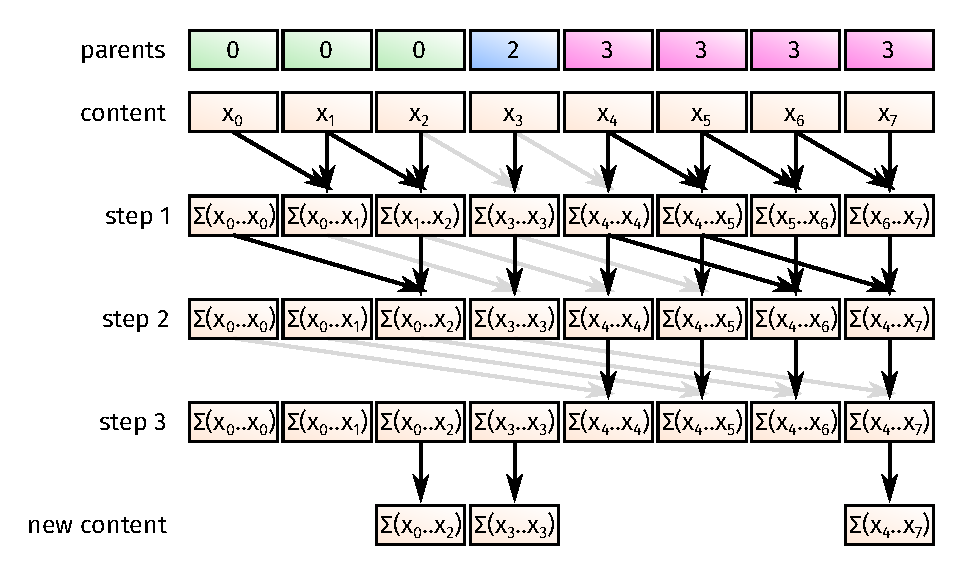
\includegraphics[width=0.7\linewidth]{hillis-steele-3.pdf}
%% \end{center}

%% \caption{\label{hillis-steele-3}}
%% \end{figure}

\begin{figure}
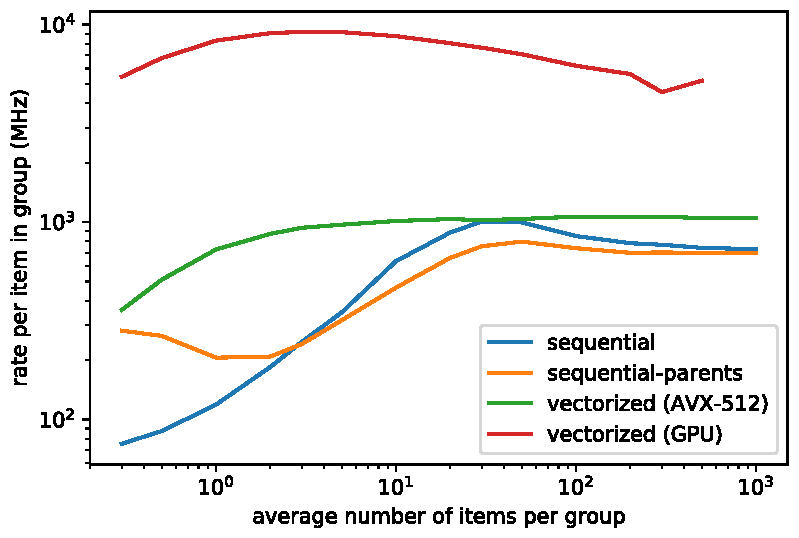
\includegraphics[width=0.5\linewidth]{sum_rates_logy.pdf}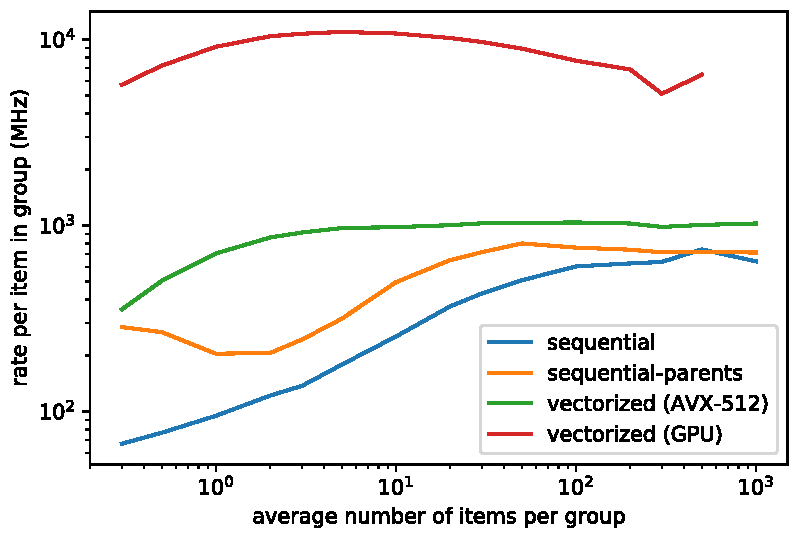
\includegraphics[width=0.5\linewidth]{max_rates_logy.pdf}

\caption{\label{rates_logy}}
\end{figure}

\section{Future directions}

Numba, Pandas, Dask, GPU

\section{Acknowledgements}

This work was supported by the National Science Foundation under grants ACI-1450377 and PHY-1624356.

\begin{thebibliography}{8}
% Journal Author, Journal \textbf{Volume}, page numbers (year)

\bibitem{uproot} Jim Pivarski et al., ``uproot'' [software], Release 3.2.6, Zenodo, 22 October, 2018. \url{https://zenodo.org/record/1469102}

\bibitem{uproot-methods} Jim Pivarski et al., ``uproot-methods'' [software], Release 0.4.1, Zenodo, 26 October, 2018. \url{https://zenodo.org/record/1472439}

\bibitem{awkward} Jim Pivarski, ``awkward-array'' [software], Release 0.4.1, Zenodo, 26 October, 2018. \url{https://zenodo.org/record/1472437}

\bibitem{ieee} FIXME: IEEE paper

\bibitem{columnar-objects} FIXME: columnar objects paper (find it in Strange Loop)

\end{thebibliography}

%%%%%%%%%%%%%%%%%%%%%%%%%%%%%%%%%%%%%%%%%%%%%%%%%%%%%%%%%%%%%%%


%% \begin{frame}[fragile]{Extension to variable-sized, nested structures}
%% \vspace{0.5 cm}
%% Logical structure: \tabto{3 cm}{\ttfamily\textcolor{black}{[\textcolor{red}{[}\textcolor{darkblue}{0, 1, 2}], \textcolor{red}{[}], \textcolor{red}{[}\textcolor{darkblue}{3, 4}], \textcolor{red}{[}\textcolor{darkblue}{5, 6, 7, 8, 9}]\textcolor{red}{]}}}

%% \vspace{0.05 cm}
%% Offsets:           \tabto{3 cm}{\ttfamily\verb|[|\textcolor{red}{0,}\verb|         |\textcolor{red}{3,}\verb|  |\textcolor{red}{3,}\verb|      |\textcolor{red}{5,}\verb|             |\textcolor{red}{10}\verb|]|}

%% \vspace{0.05 cm}
%% Content:           \tabto{3 cm}{\ttfamily\verb|[ |\textcolor{darkblue}{0, 1, 2}\verb|,       |\textcolor{darkblue}{3, 4}\verb|,   |\textcolor{darkblue}{5, 6, 7, 8, 9}\verb|]|}

%% \vspace{0.05 cm}
%% Parents:           \tabto{3 cm}{\ttfamily\verb|[ |\textcolor{darkgreen}{0, 0, 0}\verb|        |\textcolor{purple}{2, 2,}\verb|   |\textcolor{darkorange}{3, 3, 3, 3, 3}\verb|]|}

%% \vspace{0.5 cm}
%% \uncover<2->{A ``jagged array'' (content $+$ offsets and/or content $+$ parents) is a basic building block of variable-sized, nested structure.}

%% \begin{itemize}
%% \item<3-> use a jagged array as the content of another jagged array to get {\tt\small list<list<X>>}
%% \item<4-> use a fixed-size rectangular array of dimension {\tt\small N} as content to get {\tt\small list<X[N]>}
%% \item<5-> use a fixed-size rectangular array of dimension {\tt\small M} as offsets to get {\tt\small list<X>[M]}
%% \end{itemize}

%% \vspace{0.25 cm}
%% \uncover<6->{When combined with a table type (column names $\to$ arrays), this is as expressive as any combination of {\tt\small std::vector} and {\tt\small struct} (i.e.\ as expressive as ProtoBuf).}
%% \end{frame}

%% \begin{frame}{Array programming can be extended to jagged arrays}
%% \vspace{0.1 cm}
%% \begin{columns}
%% \column{1.05\linewidth}
%% \begin{itemize}\setlength{\itemsep}{0.15 cm}
%% \item Multidimensional slices: \tabto{5.5 cm}{\small \mintinline{python}{events["jets"][:, 0]}} $\to$ first jet per event
%% \item<2-> Elementwise operations: \tabto{5.5 cm}{\small \mintinline{python}{jetpt * sinh(jeteta)}} $\to$ \mbox{keep jagged structure\hspace{-1 cm}}
%% \item<3-> Broadcasting: \tabto{5.5 cm}{\small \mintinline{python}{jetphi - metphi}} $\to$ expand {\small \mintinline{python}{metphi}} from

%% \tabto{5.5 cm}one-per-event to one-per-jet before operation

%% \item<4-> Masking (list compaction): \tabto{5.5 cm}{\small \mintinline{python}{data[trigger]}} $\to$ drop whole events

%% \tabto{5.5 cm}{\small \mintinline{python}{data[jetpt > 40]}} $\to$ drop jets from events

%% \item<5-> Fancy indexing (gather/scatter): \tabto{5.5 cm}{\small \mintinline{python}{a = argmax(jetpt)}} $\to$ \mbox{\small \mintinline{python}{[[2], [], [1], [4]]}\hspace{-0.5 cm}}

%% \tabto{5.5 cm}{\small \mintinline{python}{jeteta[a]}} $\to$ \mbox{\small \mintinline{python}{[[3.6], [], [-1.2], [0.4]]}\hspace{-0.5 cm}}

%% \item<6-> Row/column commutativity \tabto{5.5 cm}{\small \mintinline{python}{events["jets"]["pt"][7, 1]}} \mbox{(all the same)\hspace{-0.5 cm}}

%% (project jagged tables to \tabto{5.5 cm}{\small \mintinline{python}{events["jets"][7]["pt"][1]}}

%% jagged arrays before indexing): \tabto{5.5 cm}{\small \mintinline{python}{events[7]["jets"]["pt"][1]}}

%% \tabto{5.5 cm}{\small \mintinline{python}{events["jets"][7, 1]["pt"]}}

%% \tabto{5.5 cm}{\small \mintinline{python}{events[7]["jets"][1]["pt"]}}

%% \item<7-> Jagged array reduction: \tabto{5.5 cm}{\small \mintinline{python}{jetpt.max()}} $\to$ array of max jet $p_T$ per event
%% \end{itemize}
%% \end{columns}
%% \end{frame}

%%%%%%%%%%%%%%%%%%%%%%%%%%%%%%%%%%%%%%%%%%%%%%%%%%%%%%%%%%%%%%%

%% \section{Appendix}
%% \tiny

%% \begin{minted}{python}
%% %%timeit
%% k = 0
%% for event in events:
%%     for muon in event:
%%         pz[k] = muon.pt * math.sinh(muon.eta)
%%         k += 1
%% \end{minted}

%% \begin{minted}{python}
%% import numba

%% @numba.jit
%% def callme(pz, events):
%%     k = 0
%%     for event in events:
%%         for muon in event:
%%             pz[k] = muon.pt * math.sinh(muon.eta)
%%             k += 1

%% %%timeit
%% callme(pz, events)
%% \end{minted}

%% \begin{minted}{python}
%% import numpy

%% %%timeit
%% pz = events["pt"] * numpy.sinh(events["eta"])
%% \end{minted}

%% \begin{minted}{python}
%% %%timeit
%% k = 0
%% for event in events:
%%     pt = event["Muon_pt"]
%%     eta = event["Muon_eta"]
%%     pz[k : k + len(pt)] = pt * numpy.sinh(eta)
%%     k += len(pt)
%% \end{minted}

%% \begin{minted}{python}
%% from math import sinh

%% events = [
%%     [],
%%     [{"pt": 129.8,
%%       "eta": -1.006,
%%       "phi": -0.581},
%%      {"pt": 73.08,
%%       "eta": -0.719,
%%       "phi": -1.51}],
%%     ...
%%     ]

%% %%timeit
%% k = 0
%% for event in events:
%%     for muon in event:
%%         pz[k] = (muon["pt"] *
%%                  sinh(muon["eta"]))
%%         k += 1
%% \end{minted}

%% \begin{minted}{python}
%% class Muon(object):
%%     __slots__ = ["pt", "eta", "phi"]
%%     def __init__(self, pt, eta, phi):
%%         self.pt = pt
%%         self.eta = eta
%%         self.phi = phi

%% events = [
%%     [],
%%     [Muon(129.8, -1.006, -0.581),
%%      Muon(73.08, -0.719, -1.51)],
%%     ...
%%     ]

%% %%timeit
%% k = 0
%% for event in asobjs:
%%     for muon in event:
%%         pz[k] = (muon.pt *
%%                  sinh(muon.eta))
%%         k += 1
%% \end{minted}

%% \begin{minted}{python}
%% import ROOT
%% import root_numpy

%% file = ROOT.TFile("NanoAOD-DYJetsToLL.root")
%% tree = file.Get("tree")

%% %%timeit
%% root_numpy.tree2array(tree, ["Muon_pt", "Muon_eta", "Muon_phi"])




%% import uproot
%% tree = uproot.open("NanoAOD-DYJetsToLL.root")["tree"]

%% %%timeit
%% pt, eta, phi = tree.arrays(["Muon_pt", "Muon_eta", "Muon_phi"], outputtype=tuple)
%% \end{minted}

%% \begin{minted}{python}
%% import math
%% import numpy
%% import ROOT

%% file = ROOT.TFile("NanoAOD-DYJetsToLL.root")
%% tree = file.Get("tree")

%% tree.SetBranchStatus("*", 0)
%% tree.SetBranchStatus("nMuon", 1)
%% tree.SetBranchStatus("Muon_pt", 1)
%% tree.SetBranchStatus("Muon_eta", 1)

%% pz = numpy.empty(552056, dtype=numpy.float32)

%% %%timeit
%% k = 0
%% for event in tree:
%%     for pt, eta in zip(event.Muon_pt, event.Muon_eta):
%%         pz[k] = pt * math.sinh(eta)
%%         k += 1
%% \end{minted}

%% \begin{minted}{c++}
%% #include <ctime>
%% #include <sys/time.h>
%% struct timeval starttime, endtime;

%% auto file = TFile::Open("NanoAOD-DYJetsToLL.root")
%% ROOT::RDataFrame rdf("tree", file);
%% TTree* tree; file->GetObject("tree", tree);   // perhaps unnecessary, but just in case...
%% tree->SetBranchStatus("*", 0);
%% tree->SetBranchStatus("nMuon", 1);
%% tree->SetBranchStatus("Muon_pt", 1);
%% tree->SetBranchStatus("Muon_eta", 1);

%% float pz[552056];
%% gettimeofday(&starttime, 0);
%% int k = 0;
%% rdf.Foreach([&k](const ROOT::VecOps::RVec<float> &Muon_pt,
%%                  const ROOT::VecOps::RVec<float> &Muon_eta) {
%%     for (int i = 0;  i < Muon_pt.size();  i++) {
%%         pz[k]= Muon_pt[i] * sinh(Muon_eta[i]);
%%         k++;
%%     }
%% }, {"Muon_pt", "Muon_eta"});
%% gettimeofday(&endtime, 0);
%% \end{minted}

%% \begin{minted}{c++}
%% #include <ctime>
%% #include <sys/time.h>
%% struct timeval starttime, endtime;

%% auto file = TFile::Open("NanoAOD-DYJetsToLL.root")
%% TTree* tree; file->GetObject("tree", tree);   // perhaps unnecessary, but just in case...
%% tree->SetBranchStatus("*", 0);
%% tree->SetBranchStatus("nMuon", 1);
%% tree->SetBranchStatus("Muon_pt", 1);
%% tree->SetBranchStatus("Muon_eta", 1);

%% TTreeReader reader("tree", file);
%% TTreeReaderArray<float> pt(reader, "Muon_pt");
%% TTreeReaderArray<float> eta(reader, "Muon_eta");

%% gettimeofday(&starttime, 0);
%% int k = 0;
%% while (reader.Next()) {
%%     for (int i = 0;  i < pt.GetSize();  i++) {
%%         pz[k] = pt[i] * sinh(eta[i]);
%%         k++;
%%     }
%% }
%% gettimeofday(&endtime, 0);
%% \end{minted}

%% \begin{minted}{c++}
%% #include <ctime>
%% #include <sys/time.h>
%% struct timeval starttime, endtime;

%% auto file = TFile::Open("NanoAOD-DYJetsToLL.root")
%% TTree* tree; file->GetObject("tree", tree);

%% UInt_t nMuon; float pts[10]; float etas[10];
%% TBranch* nbranch = tree->GetBranch("nMuon");       tree->SetBranchAddress("nMuon", &nMuon);
%% TBranch* ptbranch = tree->GetBranch("Muon_pt");    tree->SetBranchAddress("Muon_pt", pts);
%% TBranch* etabranch = tree->GetBranch("Muon_eta");  tree->SetBranchAddress("Muon_eta", etas);

%% gettimeofday(&starttime, 0);
%% int k = 0;
%% for (int i = 0;  i < 701716;  i++) {
%%     // TBranch::GetEntry, rather than TTree::GetEntry, avoids a loop over branches
%%     nbranch->GetEntry(i);    ptbranch->GetEntry(i);    etabranch->GetEntry(i);
%%     for (int j = 0;  j < nMuon;  j++) {
%%         pz[k] = pts[j] * sinh(etas[j]);
%%         k++;
%%     }
%% }
%% gettimeofday(&endtime, 0);
%% \end{minted}

\end{document}
